\section{Description Of The Algorithm}
\label{sec:Algo_desc}
In this section, given the input string $\xv$ and the query string $\yv$, we describe our algorithm that finds the matching positions $\mathcal{T}\coleq \{\tau_1, \tau_2, \cdots \tau_L\}$ with sample and time complexities that are sub-linear in $N$. The main idea here is that the correlation vector $\rv$ is sparse (upto some noise) with dominant peaks at $L$ matching positions denoted by $\mc{T}$ and noise components at $N-L$ positions where the strings do not match. 

\begin{figure}[h!]
	\begin{center}
	 	\resizebox{0.75\textwidth}{!}{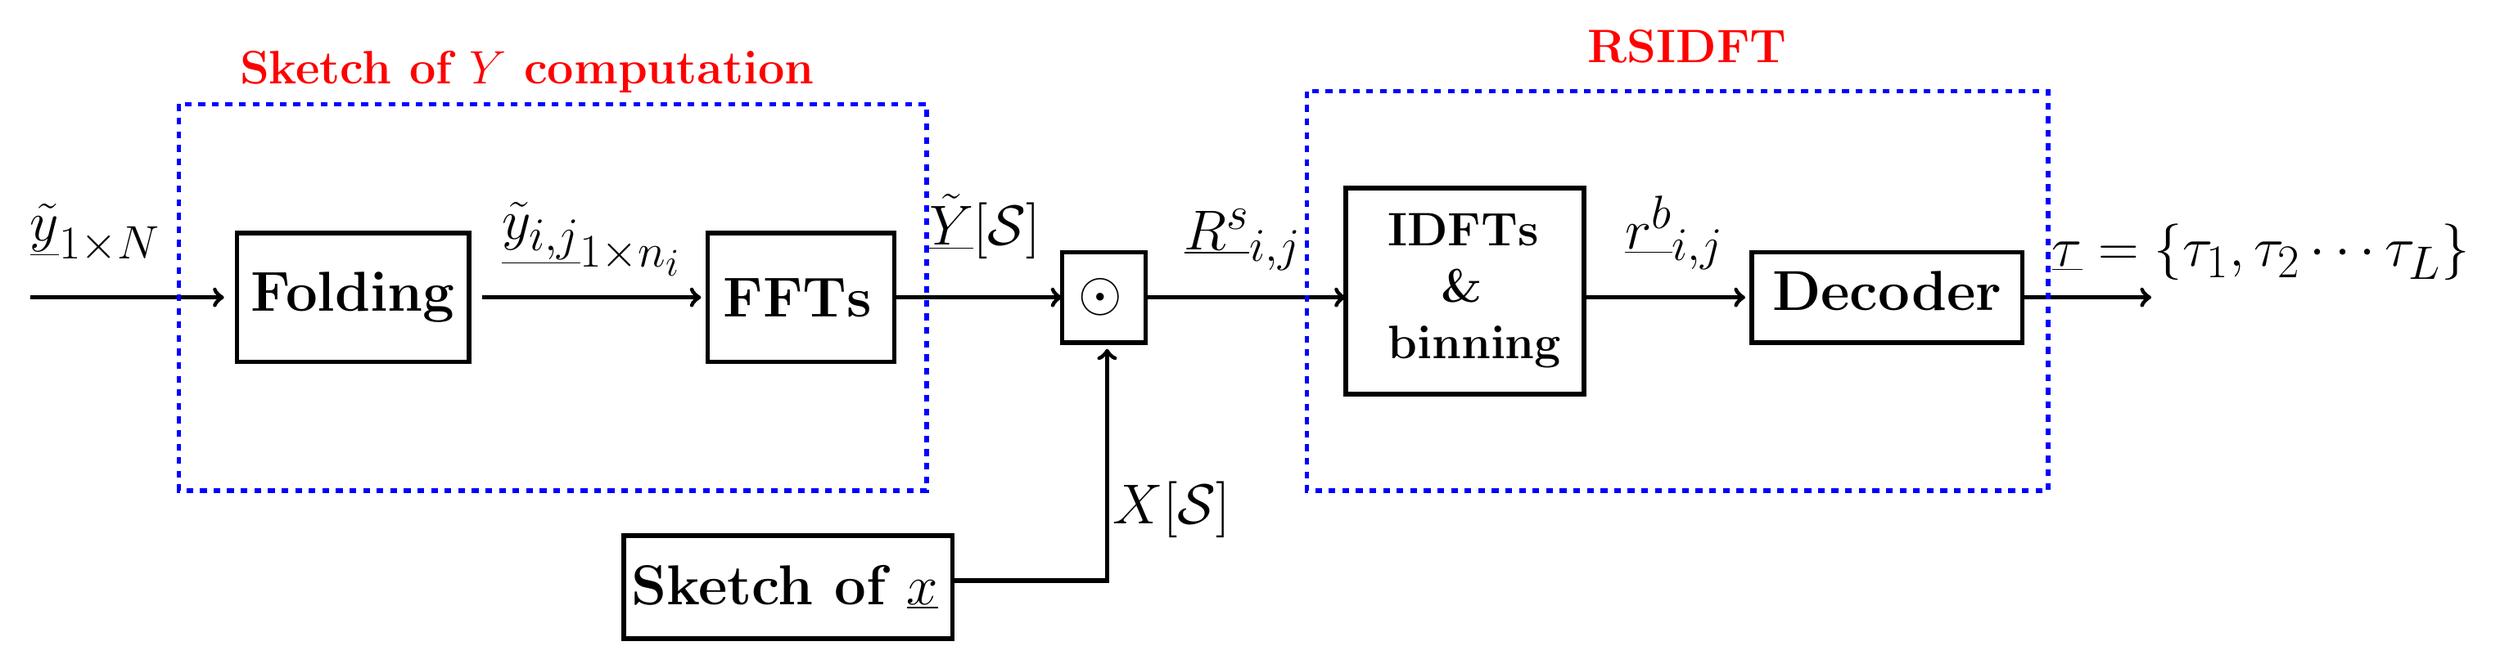
\begin{tikzpicture}

\node at (-8.7,3) { \Huge \bf  Folding};
\node at (-1.8,3) {\Huge \bf FFTs};
\node at (2.9,3) {\Huge  \bf $ \odot$};
\node [align = center] at (8.7,3.1) {\huge \bf  \begin{tabular}{l}
IDFTs \\ ~~ \& \\ binning
\end{tabular}};
\node at (-2,-1.5) { \Huge \bf Sketch of $\underline{x}$ };
\node at (15.1,3.1) {\Huge \bf  Decoder};
\draw [thick,line width =2] (-10.5,4) rectangle (-6.9,2);
\draw [thick,line width =2] (-3.2,4) rectangle (-0.3,2);
\draw [thick,line width =2] (2.3,3.7) rectangle (3.6,2.3);
\draw [thick,line width =2] (6.7,4.7) rectangle (10.4,1.5);
\draw  [thick,line width =2] (-4.5,-0.7) rectangle (0.6,-2.3);
\draw  [thick,line width =2] (13,3.7) rectangle (17.2,2.3);
\draw[->, thick, line width=2] (0.6,-1.4) -- (3,-1.4) -- (3,2.2);
\draw[->, thick, line width=2] (-6.7,3) -- (-3.3,3);
\draw[->, thick, line width=2] (-0.3,3) -- (2.3,3);
\draw [->, thick, line width=2] (3.6,3) -- (6.7,3);
\draw[->, thick, line width=2] (10.4,3) -- (12.7,3) -- (12.9,3);
\draw[->, thick, line width=2] (17.2,3) -- (19.2,3);
\draw[->, thick, line width=2] (-13.7,3) -- (-10.7,3);
\node at (-12.7,4) {\Huge$\underline{\tilde{y}}_{1 \times N}$};
\node at (-5,3.9) {\Huge$\underline{\tilde{y}_{i,j}}_{1 \times n_i}$};
\node at (11.8,4) {\Huge$\underline{r^b}_{i,j}$};
\node at (20.9,3.7) {\Huge$\underline{\tau } = \{\tau_1, \tau_2 \cdots \tau_L \}$};
\node at (4,-0.3) {\Huge $X[\mathcal{S}]$};
\node at (5.1,3.9) {\Huge $\underline{R^s}_{i,j}$};
\node at (1.1,4.1) {\Huge$\underline{\tilde{Y}}[\mathcal{S}]$};
\draw [dashed, line width =2, color=blue] (-11.4,6) rectangle (0.2,0);
\node[color= red] at (-6,6.5) {\huge \bf  Sketch of $Y$ computation};
\draw [dashed, line width =2, color=blue]  (6.1,6.2) rectangle (17.6,0);
\node [color = red] at (12,6.9) {\huge \bf RSIDFT};
\end{tikzpicture}}	
%		\includegraphics[height=3cm]{Figures/notional_diag} 
	\end{center}	   
	\caption{}\label{fig:notional}
	\vspace{5 pt}
\end{figure}

Consider the correlation signal $\rv$ in the case of exact matching:
\begin{equation} \label{eqn:RXY_sparse}
r[m] \ = \left\{
\begin{array}{ll}
  &M,~~  \text{if} \ m \in \mathcal{T} \\
  & n_m,~~ m \in [N]-\mathcal{T}
\end{array} 
\right.  
\end{equation}
where $n_m$ is the noise component that is induced due to correlation of two i.i.d. sequence of random variables each taking values from $\mathcal{A} := \{+1,-1\}$. The sparse vector $\rv$ can be computed indirectly using Fourier transform approach as shown below:
\begin{equation}\label{eqn:Rxy_fourier}
  \rv = \underset{\text{ \RNum{1} } } {\mathcal{F}_{N}^{-1}} \ \{ \underset{\text{ \RNum{2} } }{  \mathcal{F}_{N}\{\xv\}}  \odot \ \underset{\text{ \RNum{3} } }{ \mathcal{F}_{N}\{\yv'\}}  \} 
\end{equation} 
where $\mathcal{F}_{N}\{ \cdot \}$ and $\mathcal{F}_{N}^{-1}\{ \cdot \}$ refer to $N$-point discrete Fourier transform and its inverse respectively, $\odot$ is the point-wise multiplication operation and ${ y'[n]} = { y^{*}[-n]}$. Fig.~\ref{fig:notional} presents a notional schematic of our Algorithm. As evident from Eq.~\eqref{eqn:Rxy_fourier}, our algorithm for computing $\rv$ consists of three stages:
\begin{itemize}
\item Computing the sketch(FFT) $\Xv$ of $\xv$
\item Computing the sketch(FFT) $\Yv$ of $\yv$
\item Computing the IDFT of $\Rv$ given $\Xv$ and $\Yv$
\end{itemize}


	 \begin{figure}[t!]
	 	\begin{center}
	 	\resizebox{0.6\textwidth}{!}{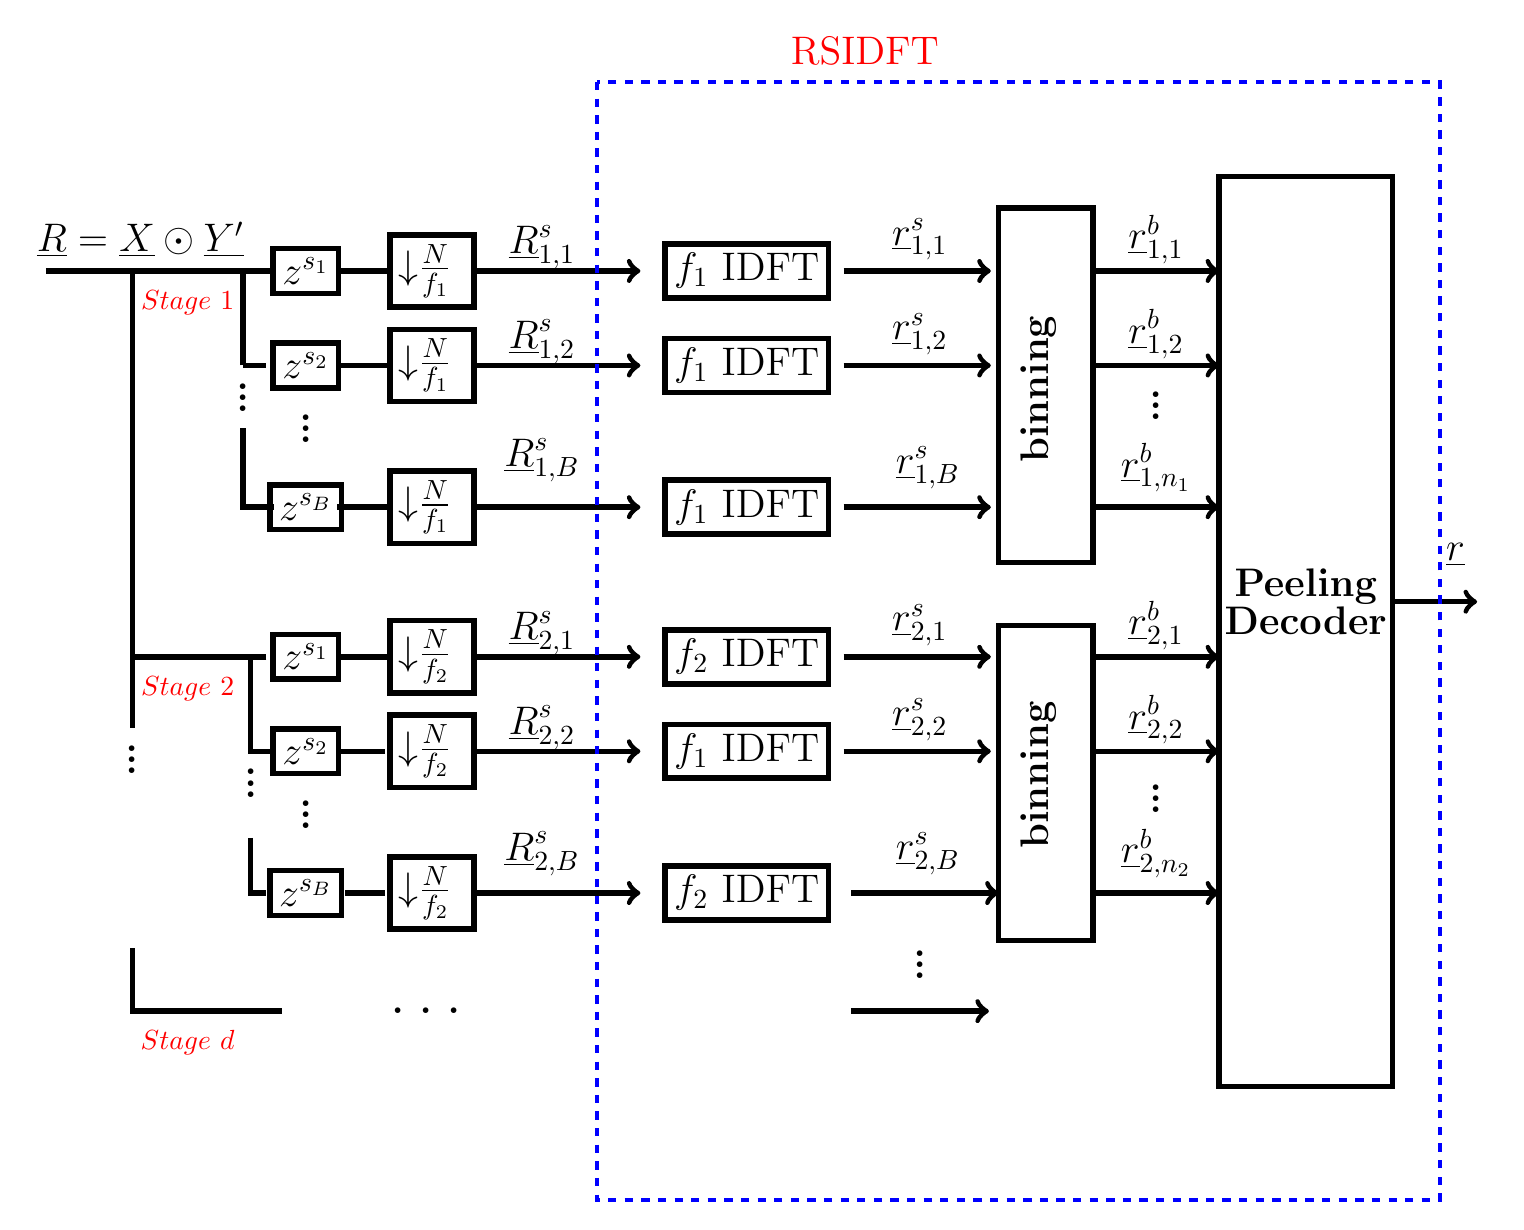
\begin{tikzpicture}

 % Downsampling blocks
\node[draw,align=center,thick,line  width =2pt] at (1.8,4.5) {\Large{$\mathbf{\downarrow} \frac{N}{f_2}$} };
\node[draw,align=center,thick,line  width =2pt] at (1.8,5.7) {\Large{$\mathbf{\downarrow} \frac{N}{f_2}$ }};
\node[draw,align=center,thick,line  width =2pt] (v6) at (1.8,2.7) {\Large{$\mathbf{\downarrow} \frac{N}{f_2}$ }};

\node[draw,align=center,thick,line  width =2pt] at (1.8,9.4) {\Large{$\mathbf{\downarrow} \frac{N}{f_1}$} };
\node[draw,align=center,thick,line  width =2pt] at (1.8,10.6) {\Large{$\mathbf{\downarrow} \frac{N}{f_1}$ }};
\node[draw,align=center,thick,line  width =2pt] at (1.8,7.6) {\Large{$\mathbf{\downarrow} \frac{N}{f_1}$ }};

%  Input lines to the down-sampling block

%  Delay blocks
\node[draw,align=center,thick,line  width =2pt] at (0.2,10.6) {\bf \Large{$z^{s_1}$}};
\node[draw,align=center,thick,line  width =2pt] at (0.2,9.4) {\bf \Large{$z^{s_2}$}};
\node[draw,align=center,thick,line  width =2pt] at (0.2,7.6) {\bf \Large{$z^{s_B}$}};

\node[draw,align=center,thick,line  width =2pt] at (0.2,5.7) {\bf \Large{$z^{s_1}$}};
\node[draw,align=center,thick,line  width =2pt] at (0.2,4.5) {\bf \Large{$z^{s_2}$}};
\node[draw,align=center,thick,line  width =2pt] at (0.2,2.7) {\bf \Large{$z^{s_B}$}};


% paths connecting the delay blocks  
 
 \draw[thick,line  width =2pt] (1.3,9.4) -- (0.6,9.4);
 

\node[line  width =2pt] at (-0.6,9.1) {\Huge{\vdots}};
\node[line  width =2pt] at (0.2,8.7) {\Huge{\vdots}};
\node[line  width =2pt] at (-0.5,4.2) {\Huge{\vdots}};
\node[line  width =2pt] at (0.2,3.8) {\Huge{\vdots}};

 \draw[thick,line  width =2pt] (1.3,10.6) -- (0.6,10.6);
 \draw[thick,line  width =2pt] (-0.6,9.4) -- (-0.6,10.6);
 
% paths connecting the two stages   
 \draw[thick,line  width =2pt] (-0.2,10.6) -- (-2,10.6);
 \draw[thick,line  width =2pt] (-0.6,9.4) -- (-0.3,9.4);
 \draw[thick,line  width =2pt] (-0.3,5.7) -- (-2,5.7);
 \draw[thick,line  width =2pt] (-2,5.7) -- (-2,10.6);
  \draw[thick,line  width =2pt] (-3.1,10.6) -- (-2,10.6);
  \draw[thick,line  width =2pt] (-2,5.7) -- (-2,4.8);
  
  
  % DFT blocks
\node[draw,align=center,thick,line  width =2pt] at (5.8,4.5) {\Large{$f_1$ IDFT}};
\node[draw,align=center,thick,line  width =2pt] at (5.8,5.7) {\Large{$f_2$ IDFT}};
\node[draw,align=center,thick,line  width =2pt] at (5.8,2.7) {\Large{$f_2$ IDFT}};

\node[draw,align=center,thick,line  width =2pt] at (5.8,9.4) {\Large{$f_1$ IDFT}};
\node[draw,align=center,thick,line  width =2pt] at (5.8,10.6) {\Large{$f_1$ IDFT}};
\node[draw,align=center,thick,line  width =2pt] at (5.8,7.6) {\Large{$f_1$ IDFT}};
% Connectors
 \draw[->,thick,line  width =2pt] (2.35,10.6) -- (4.45,10.6);
 \draw[->,thick,line  width =2pt] (2.35,9.4) -- (4.45,9.4);
 \draw[->,thick,line  width =2pt] (2.35,7.6) -- (4.45,7.6);
 
 \draw[->,thick,line  width =2pt] (2.35,5.7) -- (4.45,5.7);
 \draw[->,thick,line  width =2pt] (2.35,4.5) -- (4.45,4.5);
 \draw[->,thick,line  width =2pt] (2.35,2.7) -- (4.45,2.7);

 \draw[->,thick,line  width =2pt] (10.23,10.6) -- (11.8,10.6);
 \draw[->,thick,line  width =2pt] (10.23,9.4) -- (11.8,9.4);
 \draw[->,thick,line  width =2pt] (10.23,7.6) -- (11.8,7.6);
 
 \draw[->,thick,line  width =2pt] (10.23,5.7) -- (11.8,5.7);
 \draw[->,thick,line  width =2pt] (10.23,4.5) -- (11.8,4.5);
 \draw[->,thick,line  width =2pt] (10.23,2.7) -- (11.8,2.7);
 
  \draw[->,thick,line  width =2pt] (7.03,10.6) -- (8.9,10.6);
 \draw[->,thick,line  width =2pt] (7.03,9.4) -- (8.9,9.4);
 \draw[->,thick,line  width =2pt] (7.03,7.6) -- (8.9,7.6);
 
 \draw[->,thick,line  width =2pt] (7.03,5.7) -- (8.9,5.7);
 \draw[->,thick,line  width =2pt] (7.03,4.5) -- (8.9,4.5);
 \draw[->,thick,line  width =2pt] (7.13,2.7) -- (9,2.7);
 
  % Labels
  \node[draw=none,align=center] at (-1.9,11) {\Large{$\underline{R}= \underline{X} \odot \underline{Y'}$}};
  
  \node[draw=none,align=center] at (3.2,10.9) {\Large{$\underline{R}^{s}_{1,1}$}};
  \node[draw=none,align=center] at (3.2,9.7) {\Large{$\underline{R}^{s}_{1,2}$}};
\node[draw=none,align=center] at (3.2,8.2) {\Large{$\underline{R}^{s}_{1,B}$}};

\node[draw=none,align=center] at (3.2,6) {\Large{$\underline{R}^{s}_{2,1}$}};
  \node[draw=none,align=center] at (3.2,4.8) {\Large{$\underline{R}^{s}_{2,2}$}};
  \node[draw=none,align=center] at (3.2,3.2) {\Large{$\underline{R}^{s}_{2,B}$}};

  \node[draw=none,align=center] at (8,11) {\Large{$\underline{r}^{s}_{1,1}$}};
  \node[draw=none,align=center] at (8,9.8) {\Large{$\underline{r}^{s}_{1,2}$}};
  \node[draw=none,align=center] at (8.1,8.1) {\Large{$\underline{r}^{s}_{1,B}$}};
  
    \node[draw=none,align=center] at (11,11) {\Large{$\underline{r}^{b}_{1,1}$}};
  \node[draw=none,align=center] at (11,9.8) {\Large{$\underline{r}^{b}_{1,2}$}};
  \node[draw=none,align=center] at (11,8.1) {\Large{$\underline{r}^{b}_{1,n_1}$}};
  
     \node [draw=none] at (11,9) {\Huge{\vdots}} ;
   
  \node[draw=none,align=center] at (8,6.1) {\Large{$\underline{r}^{s}_{2,1}$}};
  \node[draw=none,align=center] at (8,4.9) {\Large{$\underline{r}^{s}_{2,2}$}};
  \node[draw=none,align=center] at (8.1,3.2) {\Large{$\underline{r}^{s}_{2,B}$}};
  
  \node [draw=none] at (11,4) {\Huge{\vdots}} ;
  
    \node[draw=none,align=center] at (11,6.1) {\Large{$\underline{r}^{b}_{2,1}$}};
  \node[draw=none,align=center] at (11,4.9) {\Large{$\underline{r}^{b}_{2,2}$}};
  \node[draw=none,align=center] at (11,3.2) {\Large{$\underline{r}^{b}_{2,n_2}$}};
  
  \node [draw=none] at (-2,4.5) {\Huge{\vdots}} ;
  
   \node[draw=none,align=center] at (-1.3,10.2) {\color{red}$Stage ~1$};
  \node[draw=none,align=center] at (-1.3,5.3) {\color{red}$Stage ~2$};
   \node[draw=none,align=center] at (-1.3,0.8) {\color{red}$Stage ~d$};
\draw [thick,line  width =2pt](-2,2) -- (-2,1.2) -- (-0.1,1.2) ;
 \node[draw=none,align=center] at (1.8,1.2) {\Huge{\ldots}};
 
\draw [thick,line  width =2pt] (11.8,0.2424) rectangle (14,11.8);
\node (v1) at (7,1.2) {};
\node (v2) at (9,1.2) {};



\node (v11) at (1.3,7.6) {};


\draw  [->,thick,line  width =2pt](v1) edge (v2);
\node at (8,1.9) {\Huge{\vdots}};
\node [text width=3cm, align =center ] at (12.9,6.4) {\Large \bf Peeling \\ Decoder};
\node (v3) at (13.9,6.4) {};
\node (v4) at (15.2,6.4) {};
\draw [thick, ->,line  width =2pt] (v3) edge (v4);
\node at (14.8,7) {\Large{$\underline{r}$}};

\draw[thick,line  width =2pt] (-0.6,8.6) -- (-0.6,7.6) -- (-0.2,7.6);
\draw[thick,line  width =2pt] (0.6,7.6) -- (1.3,7.6);
\draw[thick,line  width =2pt] (-0.5,5.7) -- (-0.5,4.5) -- (-0.2,4.5);
\draw[thick,line  width =2pt] (-0.5,3.4) -- (-0.5,2.7) -- (-0.3,2.7);
\draw [thick,line  width =2pt](0.6,5.7) -- (1.3,5.7);
\draw[thick,line  width =2pt] (0.6,4.5) -- (1.2,4.5);
\draw[thick,line  width =2pt] (0.7,2.7) -- (1.2,2.7);
\draw [dashed, color=blue, line width =1.5pt ] (3.9,13) rectangle (14.6,-1.2);
\node[color =red] at (7.3,13.4) {\Large RSIDFT  };
\draw [thick, line width =2pt]  (9,11.4) rectangle (10.2,6.9);
\draw [thick, line width =2pt]  (9,6.1) rectangle (10.2,2.1);
\node[rotate=90] at (9.5,9.1) {\Large \bf binning};
\node[rotate=90] at (9.5,4.2) {\Large \bf binning};
\end{tikzpicture}}
%	 		\includegraphics[height=7cm]{Figures/FFAST_Robust} 
	 	\end{center}	   
	 	\caption{ RSIDFT Framework to compute inverse Fourier Transform of a signal $\Rv$ that is sparse in time domain. }\label{fig:rsidft}
	\vspace{5 pt}
	 \end{figure}

\subsection{Sparse Inverse Discrete Fourier Transform}
\label{subsec:RSIDFT}	
 In this section we present Robust Sparse Inverse Discrete Fourier Transform(RSIDFT) scheme that exploits sparsity in the cross-correlation signal $\rv$ and efficiently recovers it's $L$ dominant coefficients. The architecture of RSIDFT is similar to that of the FFAST scheme proposed in \cite{pawar2014robust}, but the decoding algorithm has some key modifications to handle the noise model induced in this problem. We will see in Sec.~\ref{subsec:skteches} how the sketches $\Xv$ and $\Yv$ are computed efficiently but for this section we will focus only on the recovery of the sparse coefficients in $\rv$ given $\Xv$ and $\Yv$.
	  	  
Consider the RSIDFT framework shown in Fig.~\ref{fig:rsidft}. Let $ \Rv =\Xv \odot \Yv'$ be the DFT of the cross-correlation signal of $\xv$ and $\yv$. The framework consists of {\it $d$-stages} with each stage correpsonding to a sub-sampling factor of $\frac{N}{f_i}$. The design scheme for choosing parameters $\{f_1,f_2,\ldots,f_d\}$ for various values of $\mu$ such that $f_i | N$ and $f_i=N^{\alpha}+O(1) \forall ~i\in[d]$ are given in \ref{subsec:DesignParameters}. In each stage, there are {\it $B$ branches} with shifts from the set $ \{s_1, s_2, \cdots s_B\} $, where $s_1 =0$ in the first branch and the rest are chosen randomly from $[N]$.
	   	 	
	 Given the input $\Rv$, in branch $j$ of $i^{\text{th}}$ stage of RSDIFT, referred to as \textit{branch $(i,j)$} for simplicity, RSIDFT sub-samples the signal $\Rv$ at
\begin{align}
\label{Eqn:SamplingSets}
	 \mathcal{S}_{i,j} \coleq \{s_j,\ s_j + n_i,\ s_j + 2n_i,\ \cdots s_j + (f_i-1) n_i\}, \quad i\in[d], j\in[B]
\end{align}
where $n_i\coleq \frac{N}{f_i}$ to obtain $\Rv_{i,j}\coleq\Rv[\mc{S}_{i,j}]$. The sub-sampling operation is followed by a $f_i$-point IDFT in each branch of stage-$i$ to obtain $ \rv_{i,j}$. Notice that $ \rv_{i,j}$ is an aliased version of $\rv$ due to the property that sub-sampling in Fourier domain is equivalent to aliasing in time domain.

	 Let $\zv_{i,k}\in\mbb{R}^{B}$, for $k\in [f_i]$, be the $k$th \textit{binned} observation vector of stage-$i$ formed by stacking $\rv_{i,j}[k], j\in[B]$, together as a vector i.e.
\[
	  \zv_{i,k} = \begin{bmatrix}
	 r_{i,1}[k] \\
	 r_{i,2}[k] \\
	 \vdots\\
	 r_{i,B}[k]
	 \end{bmatrix}  
\]
Using the properties of Fourier transfrom, we can write the relationship between the observation vectors $\zv_{i,j}$ at bin $(i,j)$ and sparse vector to be estimated $\rv$ as:
\begin{align}
	\label{Eqn:Generator Equation}
	\zv_{i,k}= \mb{W}_{i,k} \times
	\begin{bmatrix}
		r[k+(0)f_i] \\
		r[k+(1)f_i] \\
		\vdots\\
		r[k+(n_i-1)f_i]
	\end{bmatrix}
\end{align}

where we refer to $\mb{W}_{i,k}$ as the sensing matrix at bin $(i,k)$ and is defined as  
\begin{align}\label{Eqn:Sensing Matrix}
	\mb{W}_{i,k} = \left[\wv^{k},\wv^{k+f_i},\ldots, \wv^{k+(n_i-1)f_i}\right] \text{where} ~\wv^{k}=
	\begin{bmatrix}
		e^{\frac{j2\pi ks_1}{N}}\\
		e^{\frac{j2\pi ks_2}{N}}\\
		\vdots\\
		e^{\frac{j2\pi ks_B}{N}}
	\end{bmatrix}
\end{align}

\begin{figure}[h!]
	\begin{center}
%		\includegraphics[height=7cm]{Figures/Factorgraph} 
	 	\resizebox{0.75\textwidth}{!}{\begin{tikzpicture}

\definecolor{brightturquoise}{rgb}{0.03, 0.91, 0.87}
\definecolor{buff}{rgb}{0.94, 0.86, 0.51}
\definecolor{caribbeangreen}{rgb}{0.0, 0.8, 0.6}
\definecolor{celadon}{rgb}{0.67, 0.88, 0.69}
\definecolor{darktangerine}{rgb}{1.0, 0.66, 0.07}
\definecolor{darkviolet}{rgb}{0.58, 0.0, 0.83}
\definecolor{deepskyblue}{rgb}{0.0, 0.75, 1.0}
\definecolor{amber(sae/ece)}{rgb}{1.0, 0.49, 0.0}
\definecolor{antiquewhite}{rgb}{0.98, 0.92, 0.84}
\definecolor{applegreen}{rgb}{0.55, 0.71, 0.0}
\definecolor{babyblue}{rgb}{0.54, 0.81, 0.94}

\def\nodewidth{0.8in}
\tikzstyle{bit} = [circle, draw, thick,fill=gray,opacity=0.7,line width =2, minimum size=\nodewidth]

% Variable nodes 
\node[bit] (v6) at (-7,-6){};
\node[bit] (v5) at (-7,-2.2) {};
%\draw[thick,fill=gray,line width =2,opacity=0.7]  (-7,-2.2) node (v5) {} ellipse (1 and 1);
\draw [thick,fill=gray,line width =2,opacity=0.7]  (-7,1.4) node (v3) {} ellipse (1 and 1);
\draw  [thick,fill=gray,line width =2,opacity=0.7]  (-7,-9.2) node (v1) {} ellipse (1 and 1);
\draw  [thick,fill=gray,line width =2,opacity=0.7]  (-7,-12.6) node (v1_1) {} ellipse (1 and 1);
\draw  [thick,fill=gray,line width =2,opacity=0.7]  (-7,4.9) node (v1_2) {} ellipse (1 and 1);

%Check nodes
\draw [thick,line width =2] (1.7,4.5) rectangle (3.7,2.5);
\draw [thick,line width =2]  (1.7,1.5) node (v8) {} rectangle (3.7,-0.5);
\draw [thick,line width =2] (1.7,-1.5) rectangle (3.7,-3.5);
\draw [thick,line width =2] (1.7,-7.3) rectangle (3.7,-9.3);
\draw [thick,line width =2] (1.7,-10.7) rectangle (3.7,-12.7);

\node (v2) at (1.7,3.5) {};
\node (v4) at (1.7,-2.5) {};
\node (v7) at (1.7,-8.3) {};
\node (v9) at (1.7,-11.7) {};
\node (v10) at (0.5,-5.3) {};
\node (v11) at (4.4,-5.3) {};



\node at (-9.6,4.8) {\Huge $r[0]$};
\node at (-9.6,1.4) {\Huge $r[1]$};
\node at (-9.6,-2.2) {\Huge $r[2]$};
\node at (-9.6,-6) {\Huge $r[3]$};
\node at (-9.6,-9.2) {\Huge $r[4]$};
\node at (-9.6,-12.6) {\Huge $r[5]$};


\draw [dashed] (v10) edge (v11);
\node [anchor=west] at (4.6,4.2) {\Huge $ \zv_{1,1} = \begin{bmatrix}
	 r_{1,1}[1] = r[0] w_1^{0} + r[3] w_1^{3}  \\
	 r_{1,2}[1] = r[0] w_2^{0} + r[3] w_2^{3} \\
	 \end{bmatrix}$};

\node [anchor=west] at (4.6,1) {\Huge $  \zv_{1,2} = \begin{bmatrix}
	 r_{1,1}[2] = r[1] w_1^{1} + r[4] w_1^{4}\\
	 r_{1,2}[2] = r[1] w_2^{1} + r[4] w_2^{4}\\
	 \end{bmatrix}$};

\node [anchor=west] at (4.6,-2) {\Huge $  \zv_{1,3} = \begin{bmatrix}
	 r_{1,1}[3] = r[2] w_1^{2} + r[5] w_1^{5} \\
	 r_{1,2}[3] = r[2] w_2^{2} + r[5] w_2^{5} \\
	 \end{bmatrix}$};

\node [anchor=west] at (4.6,-7.6) {\Huge $  \zv_{2,1} = \begin{bmatrix}
	 r_{2,1}[1]= r[0] w_1^{0} + r[2] w_1^{2} + r[4] w_1^{4} \\
	 r_{2,2}[1] = r[0] w_2^{0} + r[2] w_2^{2} + r[4] w_2^{4}\\
	 \end{bmatrix}$};

\node [anchor=west] at (4.6,-11.1){\Huge $  \zv_{2,2} = \begin{bmatrix}
	 r_{2,1}[2] =  r[1] w_1^{1} + r[3] w_1^{3} + r[5] w_1^{5} \\
	 r_{2,2}[2] =  r[1] w_2^{1} + r[3] w_2^{3} + r[5] w_2^{5} \\
	 \end{bmatrix}$};


\draw[thick,line width =2]  (v1_2) edge (v2);
\draw[thick,line width =2]  (v1_2) edge (v7);

\draw[thick,line width =2]  (v3) edge (v9);
\draw[thick,line width =2]  (v5.east) edge (v4);
\node[thick,line width =2] (v12) at (1.7,0.5) {};
\draw[thick,line width =2]  (v3) edge (v12);
\draw[thick,line width =2]  (v5.east) edge (v7);

\draw[thick,line width =2]  (v6.east) edge (v2);
\draw[thick,line width =2]  (v1) edge (v12);
\draw[thick,line width =2]  (v1_1) edge (v4);
\draw[thick,line width =2]  (v6.east) edge (v9);
\draw [thick,line width =2] (v1_1) edge (v9);
\draw [thick,line width =2] (v1) edge (v7);
%\node at (6,7) {\color{blue} \Huge$w_j=e^{j \frac{2\pi s_{j}}{N} }$};
\node at (13,7) { \huge $w_i^k := \left (  e^{j \frac{2 \pi s_i}{N}}\right )^{k}$};
\end{tikzpicture}
}	
	\end{center}	   
	\caption{Example of a Tanner graph formed in a RSIDFT framework with system parameters being $d=2$, $B=2$, $N=6$, $f_1 = 2$ and $f_2=3$. The variable nodes (colored gray circles) represent the cross-correlation vector $\rv$ and the bin nodes (uncolored white boxes) represent the binned observation vector $\zv_{i,k}$. The figure also illustrates the relationship between $\zv_{i,k}$ and $\rv$.}\label{fig:factorgraph}
	\vspace{5 pt}
\end{figure}

In Fig.~\ref{fig:factorgraph} we represent the relation between the set of observation vectors $\{\zv_{i,k},i\in[1:d],k\in[f_i]\}$ and $\rv$ via an example using Tanner graph. The nodes on the left, which we refer to as {\it variable nodes}, represent the $N$ elements of vector $\rv$. Similarly the nodes on the right, which we refer to as {\it bin nodes}, represent the $\sum_{i\leq d} f_i$ sub-sensing signals. We will now describe the decoding algorithm which takes the set of observation vectors $\{\zv_{i,k},i\in[1:d],k\in[f_i]\}$ at $df_i$ bins as input and estimates the $L$-sparse $\rv$.	 

\subsubsection{Decoder}		
	Observe from the Tanner graph that the degree of each variable node is $d$ and that of each bin node at stage $i$ is $n_i$. A variable node is referred to as non-zero if it corresponds to a matching position and as zero if it corresponds to a non-matching position. Note that even though the cross-correlation vector value corresponding to a non-matching position is not exactly zero but some negligible noise value we refer to them as zero variable nodes for simplicity. We refer to a bin node as {\it zero-ton} (or $\msc{H}_z$) if the number of non-zero variable nodes connected to the bin node is zero. The {\it singleton ($\msc{H}_s$), double-ton ($\msc{H}_d$) and multi-ton ($\msc{H}_m$)} bin nodes are defined similarly where the number of non-zero variable nodes connected are one, two and greater than two, respectively. The peeling decoder has the following three steps in the decoding process.

\paragraph*{Bin Classification} In this step a bin node is classified as a zero-ton or a singleton or a multi-ton. At bin $(i,j)$ the classification is done based on  comparing the first observation $z_{i,j}[1]$, which corresponds to zero shift, with a predefined threshold. For $z_{i,j}[1]=z$, the classification at bin $(i,j)$, $\widehat{\msc{H}}_{i,j}$, can be written as follows:
\begin{align}
\label{Eqn:BinClassifApprox}
\widehat{\msc{H}}_{i,j}=
\begin{cases}
\msc{H}_z &  	 z/M < \gamma_1\\
\msc{H}_s &	  \gamma_1 < z/M < \gamma_2  \\
\msc{H}_d  &    \gamma_2  < z/M <  \gamma_3\\ 
\msc{H}_m &      z/M > \gamma_3\\
\end{cases}
\end{align}
where $(\gamma_1,\gamma_2,\gamma_3)=(\frac{1-2\eta}{2},\frac{3-4\eta}{2},\frac{5-6\eta}{2})$. Note that for the case of exact matching $\eta=0$.
\paragraph*{Singleton decoding}
 If a bin node $(i,j)$ is classified as a singleton, we need to identify the position of the non-zero variable node connected to it. This is done by correlating the observation vector $\zv_{i,j}$ with each column of the sensing matrix  $\mb{W}_{i,j} \coleq [\wv^{j},\wv^{j+n_i},\ldots,   \wv^{j+(f_i-1)n_i}]$ and choose the index that maximizes the correlation value.
\begin{align*}
 \hat{k} = \underset{k\in\{j+l n_i\}}{\argmax}~~ \zv^{\dagger}_{i,j} \wv^{k}
\end{align*}
where $\dagger$ denotes the conjugate transpose. The value of the variable node connected to the singleton bin is estimated as follows:
 $$
 \hat{r}[\hat{k}]=M(1-\eta).
 $$
 Note that for the case of exact matching we know the value to be exactly equal to $M$ which is our estimate in the case of exact matching ($\eta=0)$. But in the case of approximate matching the actual value of $r[k]\in\{M(1-2\eta),\ldots,M-1,M\}$ and our estimate $ \hat{r}[\hat{k}]=M(1-\eta)$, the mid-point of the range, although is only a loose approximate it would suffice for our purposes as we are mainly interested in recovering only the positions of matches i.e. the indices of the sparse coefficients in $\rv$.			 
\paragraph*{Peeling Process} The peeling based decoder we employ consists of finding a singleton bin, then identify the single non-zero variable node connected to the bin, decoding it's value and removing ({\it peeling off}) it's contribution from all the bin nodes connected to that variable node. The main idea behind this decoding scheme is that hopefully the peeling off operation induces at least one more singleton bin and thus the process of peeling off can be repeated iteratively. Although the main idea is similar for exact matching and the approximate matching scenarios, there are some subtle differences in their implementation.\\
{\it Exact Matching}: In the case of exact matching, we remove the decoded variable node's contribution from all the bin nodes it is connected to.\\
{\it Approximate Matching}: In this case we remove the decoded variable node's contribution only from bins that are originally a singleton or a double-ton. We do not alter the bins which are classified to be multi-tons with degree more than two.   

{\it Note:} The differences in peeling implementation for exact and approximate matching cases is because unlike exact matching the approximate matching may result in non-zero error ($e_1$) between the actual correlation value $r[k]$ and the estimate $\hat{r}[\hat{k}]$, i.e. $e_1 = |r[k]- \hat{r}[\hat{k}]|$ with $0 \leq e_1 \leq \eta M$. This may lead to error propagation if we use the same decoding scheme as in exact matching. Hence to overcome this problem we impose a constraint on the type of bin nodes participating in the peeling process. 
	
We present the overall recovery algorithm, which comprises of {\it bin classification, singleton decoding} and {\it peeling process}, in the Algorithm. \ref{Algo:decoder} pseudo-code. Note that $\msc{N}(k)$ for variable node $k$ denote it's neighborhood i.e. the set of bins connected to $k^{\text{th}}$ variable node. 

\def\gap{4pt}
\begin{algorithm}[h!]
\caption{Peeling based recovery algorithm}
\label{Algo:decoder}
\begin{algorithmic}
\State Compute $\widehat{\msc{H}}_{i,j}$ for $i\in[d], j\in[f_i]$. See Eqn. \eqref{Eqn:BinClassifApprox} \hspace{26.5ex} {\it Bin Classification}
\vspace{\gap}
\While {$\exists~ i,j:\widehat{\msc{H}}_{i,j}= \msc{H}_s$,}
\vspace{\gap}
  \State $(\hat{k},\hat{r}[\hat{k}])=${\bf Singleton-Decoder}$(\zv_{i,j})$
\vspace{\gap}
  \State Assign $\hat{r}[\hat{k}]$ to $\hat{k}^{\text{th}}$ variable node
\vspace{1.5\gap}
  \For{$(i_0,j_0)\in\msc{N}(\hat{k})$}
\vspace{\gap}
	   \State $\zv_{i_0,j_0}\gets\zv_{i_0,j_0}-\hat{r}[\hat{k}]\wv^{\hat{k}}$   \hspace{45.5ex} {\it Exact Matching}
	   \vspace{\gap}
	   \State $\zv_{i_0,j_0}\gets\zv_{i_0,j_0}-\hat{r}[\hat{k}]\wv^{\hat{k}}$   \hspace{6ex} only if $\widehat{\msc{H}}_{i_0,j_0}=\msc{H}_s$ or $\msc{H}_d$ \hspace{14ex} {\it Approximate Matching}
	   \vspace{\gap}
	   \State Re-do the bin classification for $(i_0,j_0)$ and compute $\widehat{\msc{H}}_{i_0,j_0}$
      \EndFor
\EndWhile
\end{algorithmic}
\end{algorithm}

\begin{algorithm}[h!]
\caption{Singleton-Decoder}
\label{Algo:SingletonDecoder}
\begin{algorithmic}
\State{\bf Input:} $\zv_{i,j}$
\vspace{\gap}
\State{\bf Output:} $(\hat{k},\hat{r}[\hat{k}])$
\vspace{\gap}
\State Estimate singleton index to be $ \hat{k} = \underset{k\in\{j+l n_i\}}{\argmax}\  \zv^{\dagger}_{i,j} \wv^{k}$ 
\vspace{\gap}
  \State Estimate the value to be:$$ \hat{r}[\hat{k}]=
   \begin{cases}
   M & \text{ Exact Matching case}\\
  M-K & \text{ Approximate Matching case}
  \end{cases}
  $$
%  \vspace{\gap}
%  \State\hspace{23ex}           $\hat{r}[\hat{k}]=$ \hspace{10ex} Approximate Matching case
\end{algorithmic}
\end{algorithm}

\subsubsection{Choosing $f_i$ and $\alpha$ for various $\mu$}
\label{subsec:DesignParameters}
For a given value of $\mu$, we will describe how to choose the parameters $d$ and $f_i$.\\
 {\it Exact Matching} Find $d\in \mbb{N}\backslash \{1,2\}$ such that $\mu\in(\frac{1}{d},\frac{1}{d-1}]\cup[1-\frac{1}{d-1},1-\frac{1}{d})$\\
{\it Approximate Matching}: If $\mu\in(\frac{1}{8},\frac{7}{8})$, choose $d=8$. Else find $d\geq 8$ such that $\mu\in(\frac{1}{d},\frac{1}{d-1})\cup(1-\frac{1}{d-1},1-\frac{1}{d})$
\begin{itemize}
\item Find a factorization for signal length $N=\prod_{i=0}^{d-1} \mcl{P}_i$ such that the set of integers $\{\mcl{P}_0,\mcl{P}_1,\ldots,\mcl{P}_{d-1}\}$ are pairwise co-prime and all the $\mcl{P}_i$ are approximately equal
\item More precisely, let $\mcl{P}_i=\mathbf{F}+O(1) ~\forall i$ for some value $\mathbf{F}$and choose $f_i=N/\mcl{P}_i$
\item Note that our choice of design parameters results in $\alpha=1-\frac{1}{d}$ (recall $f_i\approx N^{\alpha}$)
\end{itemize} 
To summarize our choice of design parameters: In both the exact and approximate matching cases, for any $0<\mu<1$, we choose the down-sampling factors $f_i$ to be approximately equal to $N^{\alpha}$ in all the $d$-stages where $\alpha=\frac{d-1}{d}$ satisfies:
\begin{equation}
\label{Eqn:IneqMuAlpha}
\alpha>\max(\mu,1-\mu).
\end{equation}

\subsection{Sketches of $\Xv$ and $\Yv$} 
\label{subsec:skteches}		 
 As we have already seen in Sec.~\ref{subsec:RSIDFT} the RSDIFT framework requires the values of $\Rv(=\Xv\odot \Yv)$ only at indices $\mc{S}$ or in other words we need $\Xv$ and $\Yv$ only at the indices $\mc{S}$. We assume that the sketch of $\xv$, $ \Xv[\mc{S}]= \{X[i],i\in \mc{S}\}$ is pre-computed and stored in a database.

\subsubsection*{Computing the sketch of $\yv$}: For every new query $\yv$, only $\{\Yv'[\mc{S}_{i,j}],i\in[d],j\in[B]\}$ needs to be computed where the subsets $\mc{S}_{i,j}$ are defined in Eq. \eqref{Eqn:SamplingSets}. Naively, the FFT algorithm can be used to compute $\Yv'$ and the required subset of coefficients can be taken but this is inefficient and would be of $O(N \log N)$ complexity. Instead, we observe that $\Yv'[\mc{S}_{i,j}]$ is $\Yv'$ shifted by $s_j$ and sub-sampled by a factor of $n_i$. Thus for a given $(i,j)$ this corresponds to, in time domain, a point-wise multiplication by $[1,w_{s_j},w_{s_j}^2,\ldots,w_{s_j}^{N-1}]$ followed by \textit{folding} the signal into $f_i$ number of length $\frac{N}{f_i}$ signals and adding them up resulting in a single length-$n_i$ signal denoted by $\yv'_{i,j}$. Formally the \textit{folding} operation can be described as follows:
	  \begin{equation}
	  	\yv'_{i,j} = \sum \limits_{m = 0}^{n_i-1} \yv'[mf_i:(m+1)f_i-1] \odot [w_{s_j}^{mf_i},w_{s_j}^{mf_i+1},\ldots, w_{s_j}^{(m+1)f_i-1}],\qquad w_{s_j}=e^{-\frac{j2\pi s_j}{N}}.
	  \end{equation}
 Taking $n_i$-point DFT of $\yv'_{i,j}$ produces $\Yv'[\mc{S}_{i,j}]$ i.e. $\Yv'$ sampled only at $\mathcal{S}_{i,j}$ indices which is what we need in branch $(i,j)$. To obtain all the samples in $\mathcal{S}$ required for the RSDIFT framework, the \textit{folding} technique followed by a IDFT needs to be carried out for each $(i,j)$, for $i\in[d],j\in[B]$, a total of $dB$ times $N^{1-\alpha}$-point DFT.